\let\negmedspace\undefined
\let\negthickspace\undefined
\documentclass[journal]{IEEEtran}
\usepackage[a5paper, margin=10mm, onecolumn]{geometry}
%\usepackage{lmodern} % Ensure lmodern is loaded for pdflatex
\usepackage{tfrupee} % Include tfrupee package

\setlength{\headheight}{1cm} % Set the height of the header box
\setlength{\headsep}{0mm}     % Set the distance between the header box and the top of the text

\usepackage{gvv-book}
\usepackage{gvv}
\usepackage{cite}
\usepackage{amsmath,amssymb,amsfonts,amsthm}
\usepackage{algorithmic}
\usepackage{graphicx}
\usepackage{textcomp}
\usepackage{xcolor}
\usepackage{txfonts}
\usepackage{listings}
\usepackage{enumitem}
\usepackage{mathtools}
\usepackage{gensymb}
\usepackage{comment}
\usepackage[breaklinks=true]{hyperref}
\usepackage{tkz-euclide} 
\usepackage{listings}
% \usepackage{gvv}                                        
\def\inputGnumericTable{}                                 
\usepackage[latin1]{inputenc}                                
\usepackage{color}                                            
\usepackage{array}                                            
\usepackage{longtable}                                       
\usepackage{calc}                                             
\usepackage{multirow}                                         
\usepackage{hhline}                                           
\usepackage{ifthen}                                           
\usepackage{lscape}
\begin{document}

\bibliographystyle{IEEEtran}
\vspace{3cm}

\title{4.13.16}
\author{EE25BTECH11011 - Navya}
% \maketitle
% \newpage
% \bigskip
{\let\newpage\relax\maketitle}

\renewcommand{\thefigure}{\theenumi}
\renewcommand{\thetable}{\theenumi}
\setlength{\intextsep}{10pt} % Space between text and floats
\textbf{Question}:\\
The lines $p(p^2+1)x - y+q=0$and $(p2+1)^2 x+(p^2+1) y+2q=0$ are perpendicular to a common line for
\begin{enumerate}
\begin{multicols}{2}
    \item exactly one value of p
    \item exactly two values of p
    \item more than two values of p 
    \item no value of p
\end{multicols}
\end{enumerate}

\textbf{Solution}:\\
Given lines are,
\begin{align}
& p(p^2+1)x - y + q = 0  \\
& (p^2+1)^2 x + (p^2+1)y + 2q = 0
\end{align}

The normal vectors of the lines are
\begin{align}
\vec{n_1} &= \begin{pmatrix} p(p^2+1)\\ -1 \end{pmatrix}, \quad
\vec{n_2} = \begin{pmatrix} (p^2+1)^2 \\ p^2+1 \end{pmatrix}
\end{align}

If both lines are perpendicular to a common line with normal vector $\vec{m}$, then
\begin{align}
\vec{n_1}^T \vec{m} &= 0, \\
\vec{n_2}^T \vec{m} &= 0.
\end{align}

Hence, the two equations can be written together as
\begin{align}
\begin{pmatrix}
p(p^2+1) & -1 \\
(p^2+1)^2 & p^2+1
\end{pmatrix}
\vec{m} &= \vec{0}
\end{align}

Writing the system as an augmented matrix:
\begin{align}
\left[
\begin{array}{cc|c}
p(p^2 + 1) & -1 & 0 \\
(p^2 + 1)^2 & p^2 + 1 & 0
\end{array}
\right]
\end{align}


Perform row operations to reduce to RREF:
\begin{align}
& \left[
\begin{array}{cc|c}
p(p^2 + 1) & -1 & 0 \\
(p^2 + 1)^2 & p^2 + 1 & 0
\end{array}
\right]
\xrightarrow[R_1 \to \frac{1}{p(p^2+1)} R_1]{\quad}
\left[
\begin{array}{cc|c}
1 & -\frac{1}{p(p^2+1)} & 0 \\
(p^2 + 1)^2 & p^2 + 1 & 0
\end{array}
\right] \nonumber\\
\end{align}
\begin{align}
& \xrightarrow[R_2 \to R_2 - (p^2 + 1)^2 R_1]{\quad} 
 \quad
\left[
\begin{array}{cc|c}
1 & -\frac{1}{p(p^2+1)} & 0 \\
0 & (p^2 + 1) + \frac{(p^2 + 1)^2}{p(p^2+1)} & 0
\end{array}
\right] \nonumber\\
\end{align}
\begin{align}
&=
\left[
\begin{array}{cc|c}
1 & -\frac{1}{p(p^2+1)} & 0 \\
0 & (p^2 + 1)\left(1 + \frac{1}{p}\right) & 0
\end{array}
\right] \nonumber\\
\end{align}
\begin{align}
& \xrightarrow[R_2 \to \frac{1}{(p^2 + 1)\frac{p+1}{p}} R_2]{\quad} \quad
\left[
\begin{array}{cc|c}
1 & -\frac{1}{p(p^2+1)} & 0 \\
0 & 1 & 0
\end{array}
\right] 
 \xrightarrow[R_1 \to R_1 + \frac{1}{p(p^2+1)} R_2]{\quad} \quad
\left[
\begin{array}{cc|c}
1 & 0 & 0 \\
0 & 1 & 0
\end{array}
\right]
\end{align}


 For a non-trivial solution $\vec{m} \neq \vec{0}$, the system must be \textbf{rank deficient}, meaning the second row before normalization must be zero:
 
\begin{align}
(p^2 + 1) \frac{p + 1}{p} = 0.
\end{align}

 Solve for $p$:
\begin{align}
p^2 + 1 = 0 \implies p = \pm i \quad \text{(non-real, discard)},
\end{align}

or
\begin{align}
p + 1 = 0 \implies p = -1.
\end{align}

 Check special case $p = 0$:

If $p = 0$, the matrix becomes
\begin{align}
\begin{pmatrix}
0 & -1 \\
1 & 1
\end{pmatrix}
\end{align}

which has full rank, so only the trivial solution exists.

 The only real value of $p$ such that both lines are perpendicular to a common line is
\begin{align}
\boxed{p = -1}
\end{align}


\begin{figure}[h!]
    \centering
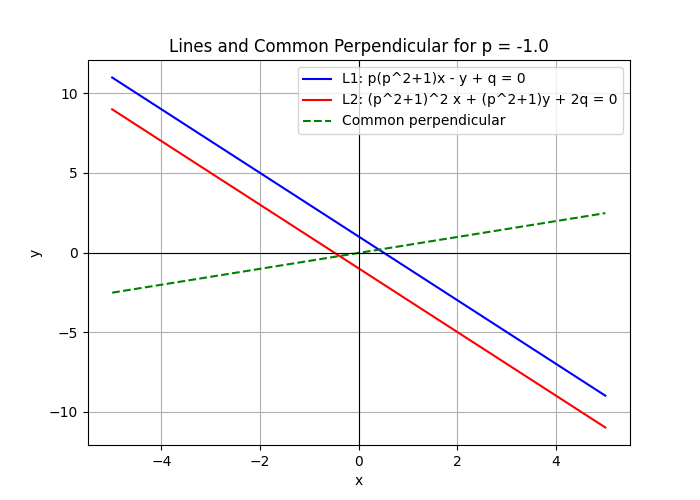
\includegraphics[width=0.8\textwidth]{figs/fig11.png}
    \label{fig:division}
\end{figure}
\end{document}